
\chapter{Syntax}
\label{syntax}

\section{Michel Chion's terminology}
\begin{itemize}
\item Added Value: sound that 'naturalises' the image
\item Anempathetic sound. Sound (usually diegetic music) that plays against the plot of the film. Chion cites a scene where a radio continues to play even when the character that turned it on has died.
\item Diegetic sound is source-visible or implied by the action of the film. It can be on-screen or off-screen.
\item Non-diegetic sound is not source-visible and is usually the musical score or additional foley/sfx to the implied (diegetic) sounds.
\item Empathetic sound is usually music that is completely within the mood of the action.
\item Reduced listening: qualitative listening independent of source or meaning (also partly quantitative). Spectral listening.
\item Semantic listening: communicative content (normally language).
\item Causal listening: listing out for source or cause (normally associated with the sound of what is seen but often used to pre-figure what is about to appear). 
\item Synchresis. Relationship between audio and visual content.
\end{itemize}

\subsection{Michel Chion \textit{Audio Vision} with examples}
\begin{itemize}
\item Eg 1. Bregman \textit{Persona, 1966}: Very complex sonically (and visually). Chion suggests watching the prologue with / without sound. 
\item Eg 2. Jacques Tati \textit{Mr. Hulot's Holiday}: Sonically very descriptive. 
\item Sound affecting the nature of time in a moving image. Sound may animate, it may accelerate, it may decimate. Chion suggests sound may \textit{vectorize} shots, directing time towards a goal.
\item Sound \textbf{unifies} the flow of images. It `bridges the visual breaks' \citep[p.47]{chion1990} 
\item Sound provides atmosphere, continuity, a background \textbf{and} a foreground. 
\item Sound \textbf{punctuates}
\item Sound \textbf{identifies} - the leitmotif.
\item Eg 3. Godard \textit{Lettre \`a Freddy Buache} \citep[p.56]{chion1990}. 
\item Sound - and silence (can you identify a passage in a film where silence was the key structural element?)
\item Sound and synch - the punch. 
\end{itemize}

First and last impressions. Try to spot a short clip (around 1 minute) with `appropriate' sounds (sfx that might `belong'). Spot a different 1 minute clip with sounds you think do not belong. Now try the inverse. On the clip with the inappropriate sounds try to re-balance the flow. It's more difficult than you think. This is because, unless you know the score, what you hear first often makes quite an indelible impression. \textit{Tip} when selecting a movie to score to \textit{do not} play the sound. You'll end up being a) tempted to score like that and b) not making as good a job. Do you own version then compare. For this you need to imagine the sounds you want to hear. 

Learn Chion's three zones \citep[p.73]{chion1990}: Onscreen sound / offscreen sound / nondiegetic sound. (73/74)
One of the most important uses of a transition between zones is, for example, nondiegetic sound gradually emerging into the scene on the radio (via a filter and amplitude change). 
Learn Chion's pit music vs. screen music. (80)
Learn Chion's Active and Passive offscreen sound. (85) 
Learn Chion's meanings of Projection. (144) 

\subsection{Post Chion: Martin Stig Andersen and \textit{Rocketman(2007)}}
\begin{itemize}
\item \url{http://www.martinstigandersen.dk/node/16}
\item \url{http://econtact.ca/12_4/andersen_audiovisual.html}
\end{itemize}

\section{Reading a film}
Refer to James Monaco's book \textit{How to read a film} \citep{monaco2000read}. 

Reading is different to watching. Reading often implies a more analytical stance. It can also imply looking through a certain lens. This can sometimes lead to a polemical or even biased response. For example you may take a feminist approach or a gendered reading. You have to be careful to remain disinterested less you read into your analysis something that isn't there (spin, obfuscation, untruths).
Notwithstanding the above, most, if not all film is a falsehood. The director has cut, edited, made numerous takes, replaced dialogue. All to fool the viewer: to pull the video world over our eyes. Look at the shot (see below section~\ref{aspects_of_footage}. The camera may be documenting; it may also be the eyes of a character. It may move or it may be static. How is the scene staged? Scenes such as `the interrogation' from \textit{Reservoir Dogs} play with the idea of off-screen action. They are all the more powerful for leaving something (not much in this case) to our imagination. 

\section{Understanding aspects of footage}
\label{aspects_of_footage}
Basic shot types include
\begin{itemize}
\item Extreme close-up (ECU)
\item Big close-up (BCU)
\item Close-up (CU)
\item Medium close-up (MCU)
\item Medium shot (MS)
\item Medium long shot (MLS)
\item Long shot (LS)
\item Very long shot (VLS)
\item Extreme long shot (ELS)
\item Two shot (2S): two people
\item Over the shoulder (OLS)
\end{itemize}

Complex shots may involve camera movement, lens adjustment as well as tracking the subject. A complex shot may pan, tilt, zoom, focus. 

\section{Harmony and Counterpoint}
\subsection{Examples and links}
\begin{itemize}
\item Some interesting examples can be found online at Rick Beato's YouTube tutorials \url{https://rickbeato.com/}. 
\item Some useful explanations of jazz harmonies can be found in The Jazz Piano Book \citep{levine2011jazz}
\item A very useful orchestration pages can be found here \url{http://andrewhugill.com/OrchestraManual/}
\end{itemize}

\subsection{Jazz chords}
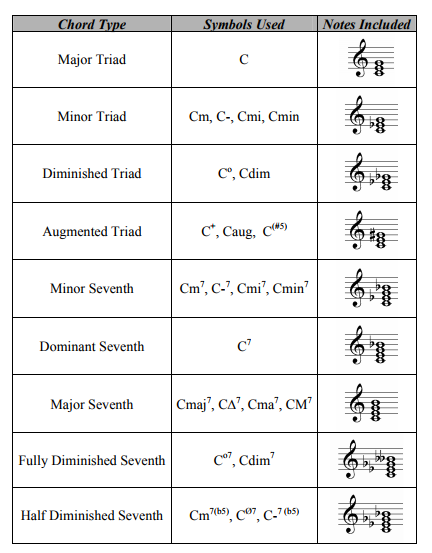
\includegraphics[scale=2.0]{jazzchords} 

\subsection{Modes}
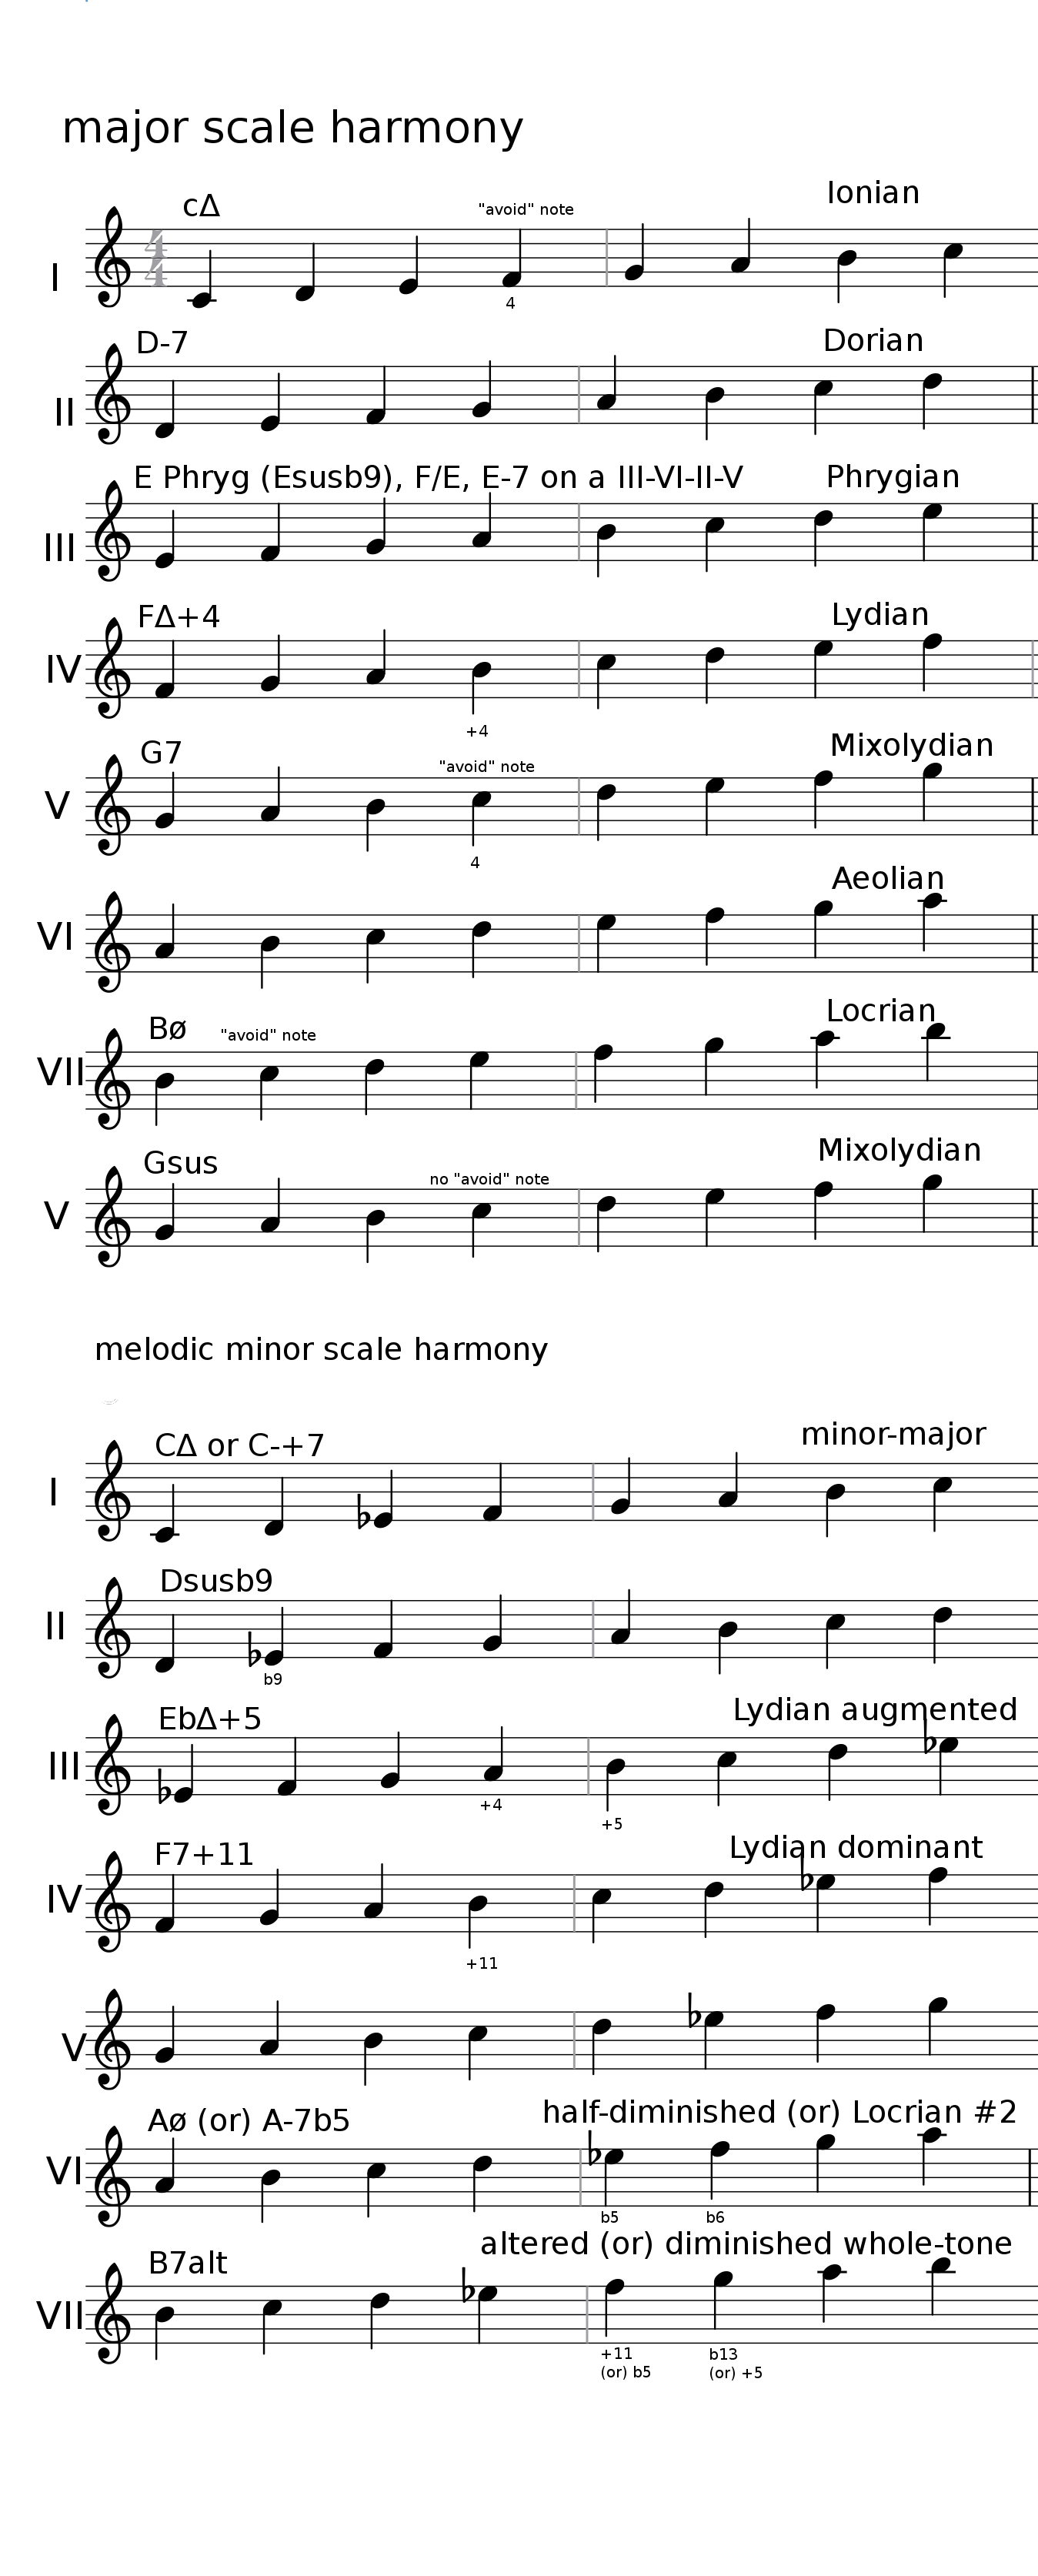
\includegraphics[scale=1.0]{modesharmony} 

\subsection{Chords in Modes}
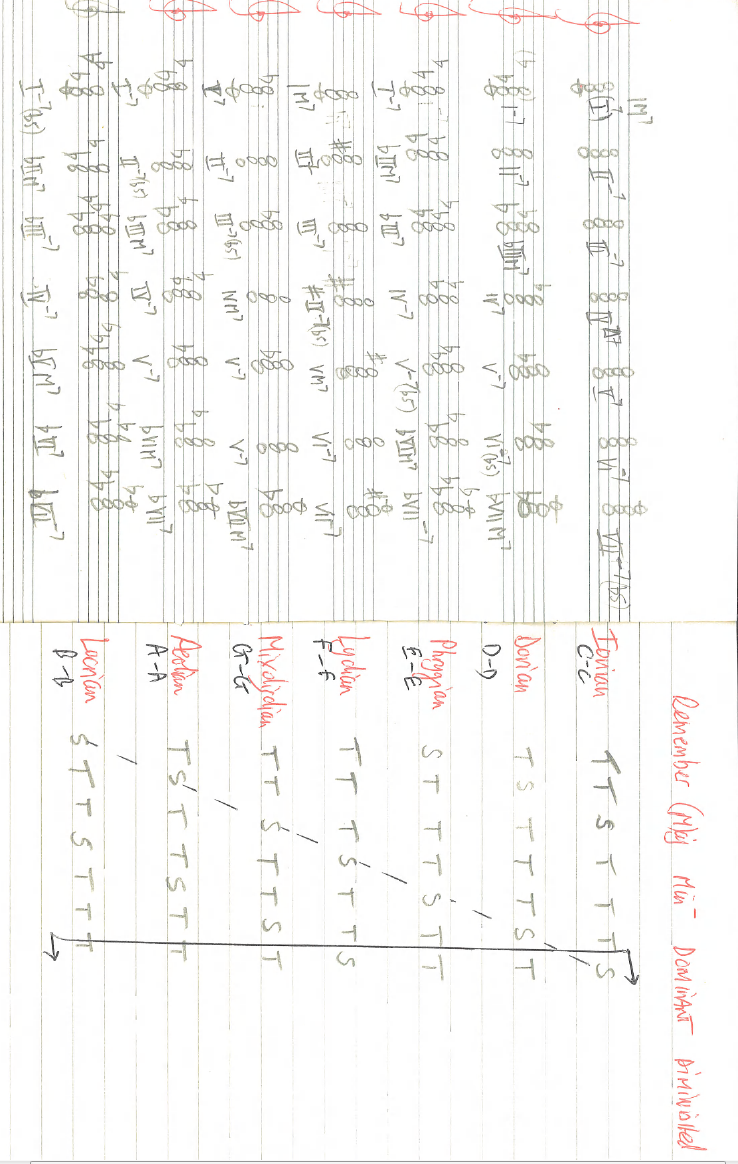
\includegraphics[scale=1.0]{chords_in_modes} 
